\documentclass{beamer}

\mode<presentation>
{
  \usetheme{Warsaw}
  % or ...
  \usecolortheme{crane}
  \setbeamercovered{transparent}
  % or whatever (possibly just delete it)
}


\usepackage[english]{babel}
% or whatever

\usepackage[utf8]{inputenc}
% or whatever

\usepackage{times}
\usepackage[T1]{fontenc}
% Or whatever. Note that the encoding and the font should match. If T1
% does not look nice, try deleting the line with the fontenc.


\title{Simulation of the Merge of Independent Chord Rings}
\author{Andrew Rosen \qquad Brendan Benshoof }
\date{} % Activate to display a given date or no date (if empty),
         % otherwise the current date is printed 
         


% If you wish to uncover everything in a step-wise fashion, uncomment
% the following command: 

%\beamerdefaultoverlayspecification{<+->}


\begin{document}

\begin{frame}
  \titlepage
\end{frame}

\begin{frame}{Outline}
  \tableofcontents
  % You might wish to add the option [pausesections]
\end{frame}

\section{Goals of Modeling and Simulation}

\subsection{Problem Space}

\begin{frame}{File Lookup}
	\begin{itemize}
		\item Most important function of a decentralized Peer-to-Peer system.
		\item Need to discover which node in the network has a certain file.
		\item Need to do it efficiently.
	\end{itemize}

\end{frame}


\begin{frame}{Hashing Protocols}
	\begin{itemize}
		\item One of the best solutions for this task.
		\item Map nodes and files identifiers to keys.
		\item Nodes are responsible for files with keys that match some criteria.
		\item Imposes an structure on the network.
	\end{itemize}

\end{frame}


\subsection{Chord}

\begin{frame}{What is Chord}
	\begin{itemize}
		\item Arranges a network into a ring.
		\item Maximum $2^m$ nodes in the network.
		\item Nodes and filenames are hashed to create an $m$-bit key.
	\end{itemize}

\end{frame}

\begin{frame}{How Are Files Stored}
\begin{center}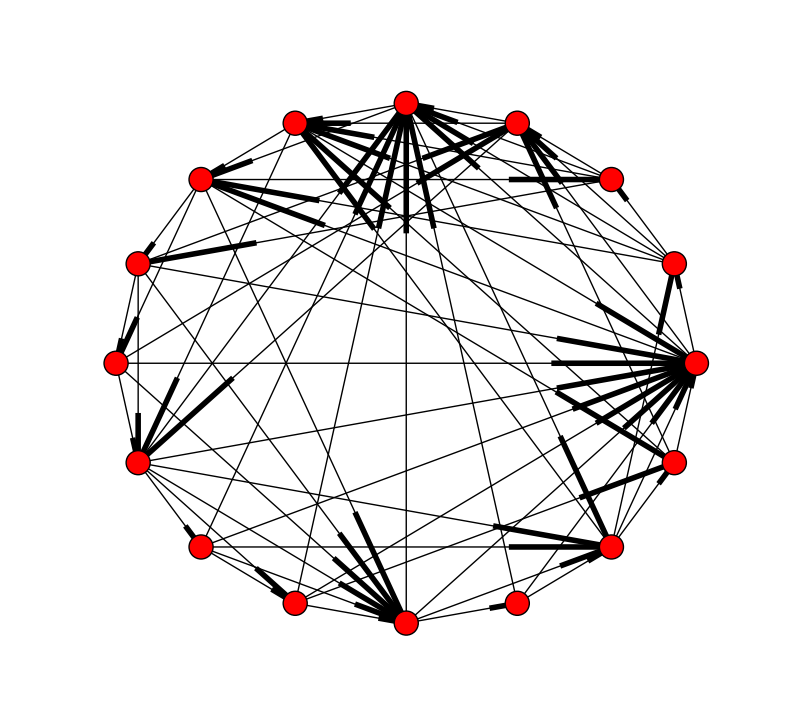
\includegraphics[scale=0.25]{chordreal}\end{center}
	\begin{itemize}
		\item Node responsible for for key $\kappa$ is the $sucessor(\kappa)$.
		\item $sucessor(\kappa)$ is the node with key $\kappa$ or first following key.
	\end{itemize}

\end{frame}


\begin{frame}{How Are Files Retrieved}
	\begin{itemize}
		\item To find a file with key $\kappa$, we find $sucessor(\kappa)$.
		\item We could just ask our successor, who would do the same.
		\item We use a \emph{finger-table} make this quicker
		\begin{itemize}
			\item $m$ entries in the table.
			\item Stores location of $successor(n+2^{i-1})$ $mod$ $2^m$.
			\item If $\kappa$ is between us and an entry, skip to that entry.
		\end{itemize}
		\item Once we know $sucessor(\kappa)$, we can directly connect.
		\item This reduces the lookup time to $O(\log n)$
	\end{itemize}

\end{frame}


\begin{frame}{How Is Churn Handled}
	\begin{itemize}
		\item Join a network by asking some node in it to find your successor.
		\item Periodically update the entries in the finger table.
		\item Periodically find your successor's predecessor.
	\end{itemize}

\end{frame}

\subsection{Goals}

\begin{frame}{Goals}
We want to examine global behavior.  As a result we ignore:
	\begin{itemize}
		\item Actual network topology outside of Chord.
		\item Real Network Latency.
		\item File storage.
	\end{itemize}
We instead focus on:
	\begin{itemize}
		\item Overlay topology.
		\item What choices are made in a race condition.
		\item What happens when rings compete for nodes.
		\item Who ends up in which ring.
	\end{itemize}

\end{frame}



\section{Developed Models} 


\subsection{Agents}
\begin{frame}{Agents}
	\begin{itemize}
		\item Nodes for nodes, Links for links.
		\item Messages are represented by:
		\begin{itemize}
			\item Seekers.
			\item Updates.
		\end{itemize}
	\end{itemize}
\end{frame}


\subsection{Simulation}

\begin{frame}{Setup}
	\begin{itemize}
		\item Generate nodes in random locations (ring visualization optional)
		\item Specified number of nodes for independent rings. 
		\item Set the hash size.
	\end{itemize}
\end{frame}

\begin{frame}{Creating Rings}
	\begin{itemize}
		\item Nodes not in a ring look within a radius for nodes in a ring
		\item Nodes then join the closest ring.
	\end{itemize}
\end{frame}


\begin{frame}{Creating Rings}
	\begin{figure}
		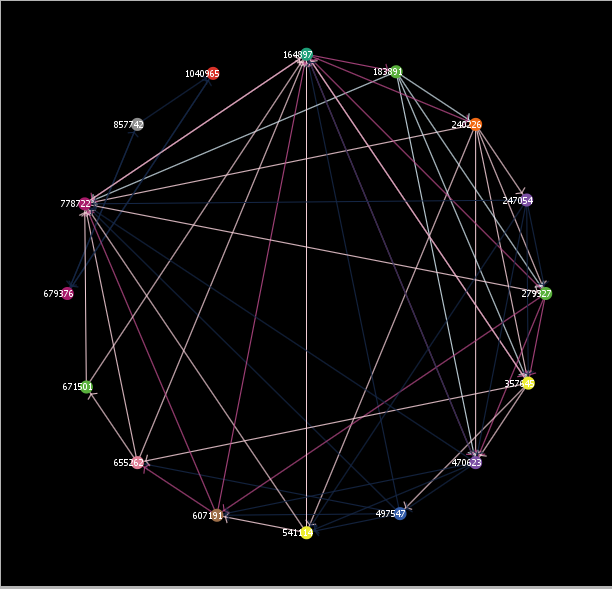
\includegraphics[scale=0.33]{example_problem}
		\caption{A chord network with multiple rings.  Rings are differentiated by color.}
		\label{problem}
	\end{figure}
\end{frame}



\subsection{Ouroboros Inaction}

\begin{frame}{Joining new Rings}
	\begin{itemize}
		\item Nodes periodically invite a new node to the ring.
		\item Nodes accept the invitation if the new ring is "better."
		\item Accepting the invitation means joining like any new node.
	\end{itemize}
\end{frame}



\section{Experiments and Results}

\subsection{Setup}

\begin{frame}{Setup}
	\begin{itemize}
		\item 200 simulations
		\begin{itemize}
			\item 100 without any joining mechanism
			\item 100 with our joining mechanism.
		\end{itemize}
		\item Recorded the number of links over time.
		\item Analyzed for the mean and variance.
	\end{itemize}
\end{frame}



\subsection{Results}

\begin{frame}{Results}
\begin{figure}
	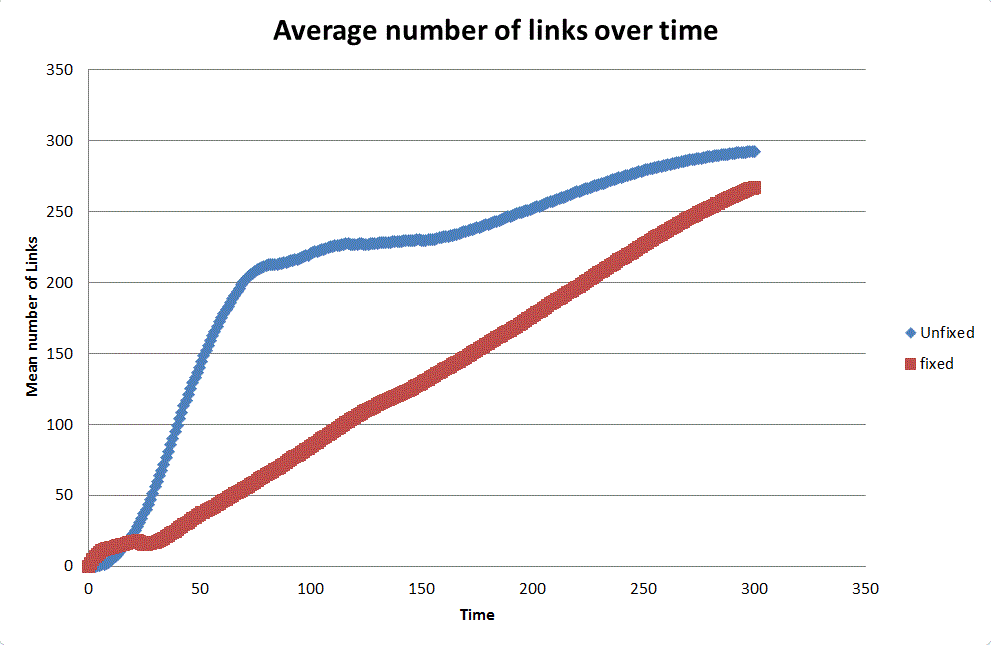
\includegraphics[scale=0.2]{chart1}
	\caption{The unfixed simulation causes nodes to form links more rapidly.  This is because nodes are not joining other rings, which would cut the number of links even as more nodes were discovered.}
	\label{chart1}
\end{figure}

\end{frame}


\begin{frame}{Results}

\begin{figure}
	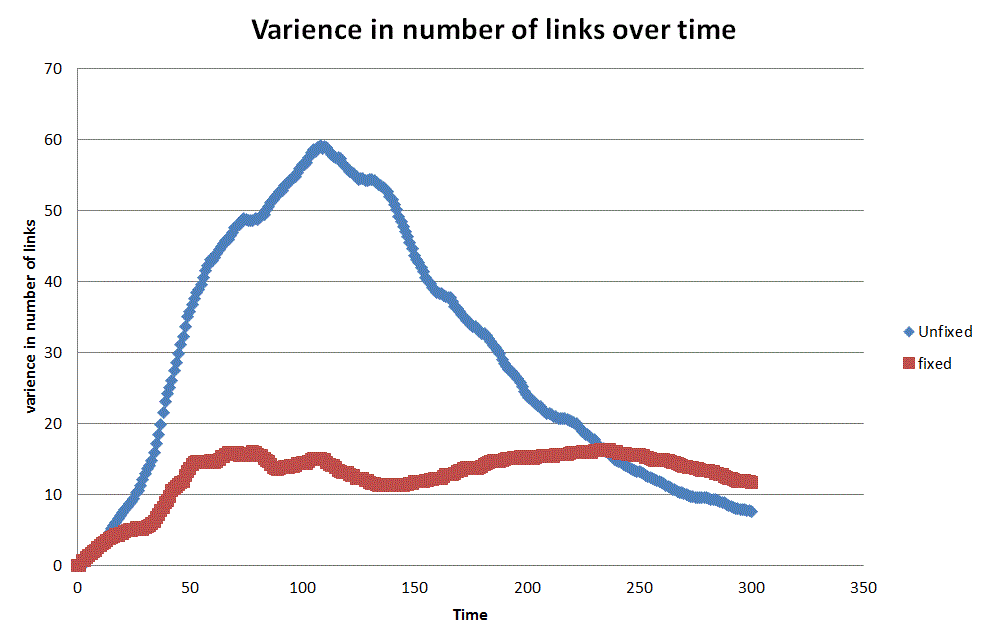
\includegraphics[width=0.7\linewidth]{chart2}
	\caption{The difference in the number of links in the rings varies wildly when nodes don't join new rings. This is expected from the extremely fast creation of links.  In the fixed network, joins keep the amount of links down to a steady number. }
	\label{chart2}
\end{figure}

\end{frame}

\section{Conclusion and Future Work}

\begin{frame}{Conclusion}
	\begin{itemize}
		\item We have a scheme to merge multiple rings.
		\item This was a necessary step for implementation.
	\end{itemize}
\end{frame}



\end{document}


